\begin{figure}[!htb]
\centering
\caption{A comparison of the formation construction in terms of graph theory metrics: connected components (A), degree (B), node connectivity (C), number of bridges (D), maximum  clique length (E), and number of colours (F).}
\begin{tikzpicture}
\begin{axis}[   ymin=0,
                ybar=0pt, 
                xticklabels={A,B,C,D,E,F},
                enlargelimits=0.15, % space between Number of Nodes (x)
                xtick=data,
                ylabel={Number of Elements},
                legend image code/.code={%
                    \draw[#1, draw=black] (0cm,-0.05cm) rectangle (0.4cm,0.1cm);
                },  
                legend style={
                    draw=black, % ?
                    text depth=0pt,
                    anchor=center,
                    at={(0.5,1)}, % space between legend and x-axis
                    legend columns=-1,
                    /tikz/every even column/.append style={column sep=0.5cm},
                },]
\addplot    +[  ybar,
                draw = black,
                fill = dark-gray,
                error bars/.cd,
                y dir=both,
                y explicit] plot
            table [x=Metric, y=Mean, y error=Interval, col sep=comma] {results/PSO/csv/score1-classic.csv};
\addplot    +[  ybar,
                draw = black,
                fill = light-gray,
                error bars/.cd,
                y dir=both,
                y explicit] plot
            table [x=Metric, y=Mean, y error=Interval, col sep=comma] {results/PSO/csv/score1-novel2.csv};
\legend{\citet{kim2018}, Proposed Approach}
\end{axis}
\end{tikzpicture}
\label{fig:PSO-graph-theory}
\imagesource{\thisauthor}
\end{figure}

%\begin{figure*}
%\centering
%    \caption{The architecture of traditional network and SDN. Source: \cite{Tang2019}}
%    \subfloat[Graph theory metrics: connected components (A), degree (B), number of bridges (C), node connectivity (D), maximum  clique length (E), and number of colours (F). ]{{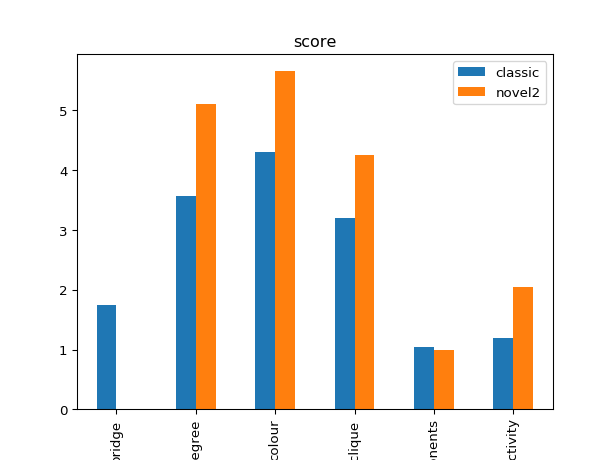
\includegraphics[scale=.4]{results/PSO/png/score.png}}}
%    \qquad
%    \subfloat[Area coverage ratio, which is the area covered by the relays over the maximum reachable area coverage having the same amount of nodes.]{{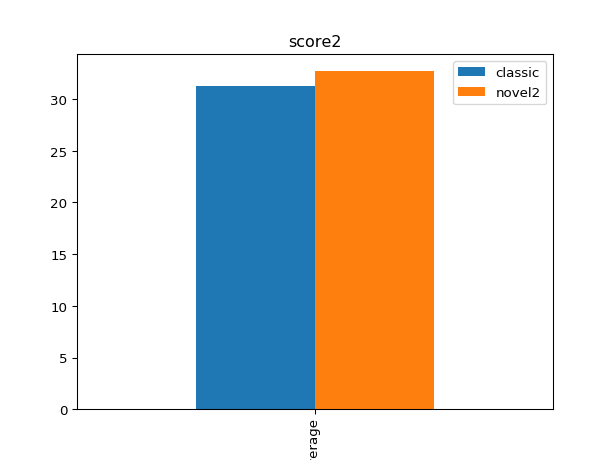
\includegraphics[scale=.4]{results/PSO/png/score2.png}}}
%	\label{figScore}
%\end{figure*}